%!Mode::"UTF-8"
\documentclass[12pt]{article}

% 页面设置
\usepackage{geometry}
\geometry{left=2.5cm, right=2.5cm, top=2.5cm, bottom=2.5cm}
\usepackage{graphicx}
\usepackage{ctex}
\usepackage{fontspec}
\usepackage{setspace}

% 代码设置
\usepackage{listings}
\usepackage{color}
\setmonofont{Consolas}
\definecolor{listing}{gray}{0.97}
\lstset{
	backgroundcolor=\color{listing},
	basicstyle=\footnotesize,
	numbers=left,
	numberstyle=\footnotesize,
	stepnumber=1,
	aboveskip={0.5\baselineskip},
	belowskip={0.5\baselineskip},
	columns=fullflexible,
	breaklines=true,
	breakatwhitespace=true,
	frame=single,
	basicstyle=\ttfamily,
	numberstyle=\ttfamily,
	tabsize=2
}

% 字体设置
\setmainfont{Times New Roman}
\setCJKmainfont{SimSun}
\setCJKsansfont{SimHei}
\usepackage[version=4]{mhchem}

% 表格设置
\usepackage{makecell}
\newcommand{\addcell}[2][4]{\makecell{\zihao{#1}\textsf{#2}}}
\usepackage{titlesec}
\usepackage{booktabs}
\usepackage{tabularx}

% 设置图注、表注
\usepackage{caption}
\usepackage{bicaption}
\captionsetup{labelsep=quad, font={small, bf}, skip=2pt}
\DeclareCaptionOption{english}[]{
    \renewcommand\figurename{Fig.}
    \renewcommand\tablename{Table}
}
\captionsetup[bi-second]{english}

% 设置页眉
\usepackage{fancyhdr}
\pagestyle{fancy}
\fancypagestyle{preContent}{
    \fancyhead[L]{\zihao{-5} 物理化学实验}
    \fancyhead[C]{\zihao{-5} 实验四\ \ 双液体系沸点-成分图的绘制}
    \fancyhead[R]{\zihao{-5} 1800011828\ 王宇哲}
}
\pagestyle{preContent}

%	设置首页页眉页脚
\fancypagestyle{plain}{
	\fancyhead[L]{\zihao{-5} 物理化学实验}
	\fancyhead[C]{\zihao{-5} 实验四\ \ 双液体系沸点-成分图的绘制}
	\fancyhead[R]{\zihao{-5} 1800011828\ 王宇哲}
	\cfoot{}
}

% 设置标题格式
\titleformat*{\section}{\zihao{4}\sffamily}
\titleformat*{\subsection}{\zihao{-4}\sffamily}
\titleformat*{\subsubsection}{\zihao{-4}\sffamily}
\titlespacing*{\section}{0pt}{10pt}{10pt}
\titlespacing*{\subsection}{0pt}{10pt}{5pt}
\titlespacing*{\subsubsection}{0pt}{10pt}{5pt}

% 设置引用格式
\usepackage[super,round,comma,compress]{natbib}

\usepackage{amsmath}
\usepackage{amssymb}

%设置封面
\begin{document}
    % 标题页
    \begin{titlepage}
    	% 页眉
    	\thispagestyle{plain}
        % 图片
        \begin{figure}[h]
            \centering
            \includegraphics{pku.png}
        \end{figure}
        \vspace{24pt}
        % 标题
        \centerline{\zihao{-0} \textsf{物理化学实验报告}}
        \vspace{40pt} % 空行
        \begin{center}
            \begin{tabular}{cp{10 cm}}
                % 题目
                \addcell[2]{题目:\ } & \addcell[2]{双液体系沸点-成分图的绘制} \\
                \cline{2-2}
            \end{tabular}
        \end{center}
        \vspace{20pt} % 空行
        \begin{center}
            \doublespacing
            \begin{tabular}{cp{5cm}}
                % 姓名
                \addcell{姓\phantom{空格}名:\ } & \addcell{王宇哲} \\
                \cline{2-2}
                % 学号
                \addcell{学\phantom{空格}号:\ } & \addcell{1800011828}\\
                \cline{2-2}
                % 组别
                \addcell{组\phantom{空格}别:\ } & \addcell{11组3号} \\
                \cline{2-2}
                % 实验日期
                \addcell{实验日期:\ } & \addcell{2020.12.9}\\
                \cline{2-2}
                % 室温
                \addcell{室\phantom{空格}温:\ } & \addcell{291.75\ K}\\
                \cline{2-2}
                % 大气压强
                \addcell{大气压强:\ } & \addcell{101.97\ kPa}\\
                \cline{2-2}
            \end{tabular}
            \begin{tabular*}{\textwidth}{c}
                \\ % 这是空行
                \\ % 这是空行
                \\ % 这是空行
                \\ % 这是空行
                \hline % 分割线
            \end{tabular*}
        \end{center}
        % 摘要
        \textsf{摘\ \ 要}\ \ 本实验采用回流冷凝法测定了不同浓度乙醇-环己烷体系的沸点和气相、液相折射率,作出$n-\chi_{\ce{EtOH}}$工作曲线,计算了各平衡沸点下的两相组成,绘制了乙醇-环己烷体系沸点-成分图,确定了恒沸点$t_{b}=64.97\ \ {\rm ^{\circ}C}$,组成为$\chi_{\ce{EtOH}}=0.31$,并讨论了插值和拟合作出标准工作曲线的区别、标准工作曲线非直线的原因。
        \\
        \\
        % 关键字
        \textsf{关键词}\ \ 环己烷-乙醇体系;气液平衡;沸点-成分图;折射率
    \end{titlepage}

    \section{引言}
	略
               
\vbox{}        
    \section{实验部分}
    	\subsection{仪器和试剂}
环己烷(AR),乙醇(AR);\par 
恒沸点仪,阿贝折射仪,变压器,$4\ \ \Omega$电阻丝,$1/10$刻度温度计,试管,小滴瓶,$1\ \ {\rm mL}$移液管,$5\ \ {\rm mL}$移液管,$20\ \ {\rm mL}$移液管,蒸馏烧瓶。
     
\vbox{}
    	 \subsection{实验内容\citealp{physchemlab}}
			\subsubsection{沸点和两相成分的测定}
		洗净、烘干蒸馏瓶,加入$20\ \ {\rm mL}$乙醇,装好仪器,温度计的水银球$1/2$浸入液体内,冷凝管内通入冷水。将电阻丝接在输出电压$12.6\ \ {\rm V}$的变压器上,使温度升高并沸腾。待温度稳定后数分钟,记下温度及大气压。切断电源,用两支干净的滴管,分别取出支管处的气相冷凝液和蒸馏瓶中的液体几滴,立即使用阿贝折射仪测定其折射率。 \par 
		蒸馏瓶中加入$1\ \ {\rm mL}$环己烷,按前述方法测定平衡沸点$t_{b}$及气相折射率$n^{g}$、液相折射率$n^{l}$。再依次加入$1.00\ \ {\rm mL}$、$2.00\ \ {\rm mL}$、$3.00\ \ {\rm mL}$、$3.00\ \ {\rm mL}$、$4.00\ \ {\rm mL}$、$5.00\ \ {\rm mL}$环己烷,记录液体组成,进行同样的实验。\par
		上述实验结束后,回收母液,再用少量环己烷洗$3\sim 4$次蒸馏瓶,注入$20.00\ \ {\rm mL}$环己烷,再装好仪器。先测定纯环己烷的沸点,然后依次加入$0.20\ \ {\rm mL}$、$0.20\ \ {\rm mL}$、$0.50\ \ {\rm mL}$、$0.50\ \ {\rm mL}$、$2.00\ \ {\rm mL}$、$2.00\ \ {\rm mL}$、$5.00\ \ {\rm mL}$、$5.00\ \ {\rm mL}$乙醇,分别测定平衡沸点$t_{b}$及气相折射率$n^{g}$、液相折射率$n^{l}$。
		
\subsubsection{标准工作曲线绘制}
	洗净并烘干$6$个小滴瓶,冷却后准确称量其质量$m_{0}$。用带刻度的移液管分别加入$1.00\ \ {\rm mL}$、$2.00\ \ {\rm mL}$、$3.00\ \ {\rm mL}$、$4.00\ \ {\rm mL}$、$5.00\ \ {\rm mL}$、$6.00\ \ {\rm mL}$乙醇,分别称量其质量$m_{1}$,再依次分别加入$6.00\ \ {\rm mL}$、$5.00\ \ {\rm mL}$、$4.00\ \ {\rm mL}$、$3.00\ \ {\rm mL}$、$2.00\ \ {\rm mL}$、$1.00\ \ {\rm mL}$环己烷,再分别称量其质量$m_{2}$,旋紧盖子后摇匀。\par 
	在恒温$t=30.0\ \ {\rm ^{\circ}C}$下分别测定这些样品的折射率$n$。



\vbox{}
 \section{数据与结果}
 \subsection{实验数据记录及处理}
 \subsubsection{乙醇中加入环己烷体系沸点和两相成分的测定}
 测定乙醇中加入环己烷体系的平衡沸点$t_{b}$及气相折射率$n^{g}$、液相折射率$n^{l}$,记录液体的组成,结果如\textbf{表1}所示。
\begin{table}[h]
	\centering
	\zihao{5}
	\bicaption{乙醇中加入环己烷体系沸点及折射率测定实验数据}{Experimental data of boiling point and refractive index of ethanol with cyclohexane}
	\begin{tabular}{ccccc}
		\toprule
		编号 & 组分 & $t_{b}/{\rm ^{\circ}C}$& $n^{l}$ & $n^{g}$ \\
		\midrule
		1 & $20.00\ \ {\rm mL\ \ } \ce{EtOH}$ & 78.19 & 1.3584 & 1.3582 \\
		2 & $20.00\ \ {\rm mL\ \ } \ce{EtOH}$及$1.00\ \ {\rm mL\ \ } \ce{Cy}$  & 75.30 & 1.3601 & 1.3746 \\
		3 & $20.00\ \ {\rm mL\ \ } \ce{EtOH}$及$2.00\ \ {\rm mL\ \ } \ce{Cy}$  & 73.35 & 1.3632 & 1.3850 \\
		4 & $20.00\ \ {\rm mL\ \ } \ce{EtOH}$及$4.00\ \ {\rm mL\ \ } \ce{Cy}$  & 70.45 & 1.3668 & 1.3915 \\
		5 & $20.00\ \ {\rm mL\ \ } \ce{EtOH}$及$7.00\ \ {\rm mL\ \ } \ce{Cy}$  & 67.92 & 1.3732 & 1.3950 \\
		6 & $20.00\ \ {\rm mL\ \ } \ce{EtOH}$及$11.00\ \ {\rm mL\ \ } \ce{Cy}$  & 66.43 & 1.3773 & 1.3964 \\
		7 & $20.00\ \ {\rm mL\ \ } \ce{EtOH}$及$16.00\ \ {\rm mL\ \ } \ce{Cy}$  & 65.72 & 1.3836 & 1.3977 \\
		\bottomrule
	\end{tabular}
\end{table}
\par


\subsubsection{环己烷中加入乙醇体系沸点和两相成分的测定}
测定环己烷中加入乙醇体系的平衡沸点$t_{b}$及气相折射率$n^{g}$、液相折射率$n^{l}$,记录液体的组成,结果如\textbf{表2}所示。
\begin{table}[h]
	\centering
	\zihao{5}
	\bicaption{环己烷中加入乙醇体系沸点及折射率测定实验数据}{Experimental data of boiling point and refractive index of cyclohexane with ethanol}
	\begin{tabular}{ccccc}
		\toprule
		编号 & 组分 & $t_{b}/{\rm ^{\circ}C}$& $n^{l}$ & $n^{g}$ \\
		\midrule
		1 & $20.00\ \ {\rm mL\ \ } \ce{Cy}$ & 80.30 & 1.4218 & 1.4216 \\
		2 & $20.00\ \ {\rm mL\ \ } \ce{Cy}$及$0.20\ \ {\rm mL\ \ } \ce{EtOH}$  & 78.29 & 1.4206 & 1.4024 \\
		3 & $20.00\ \ {\rm mL\ \ } \ce{Cy}$及$0.40\ \ {\rm mL\ \ } \ce{EtOH}$  & 74.16 & 1.4201 & 1.4007 \\
		4 & $20.00\ \ {\rm mL\ \ } \ce{Cy}$及$0.90\ \ {\rm mL\ \ } \ce{EtOH}$  & 68.21 & 1.4185 & 1.3999 \\
		5 & $20.00\ \ {\rm mL\ \ } \ce{Cy}$及$+1.40\ \ {\rm mL\ \ } \ce{EtOH}$  & 66.68 & 1.4168 & 1.3995 \\
		6 & $20.00\ \ {\rm mL\ \ } \ce{Cy}$及$3.40\ \ {\rm mL\ \ } \ce{EtOH}$  & 65.22 & 1.4106 & 1.3990 \\
		7 & $20.00\ \ {\rm mL\ \ } \ce{Cy}$及$8.40\ \ {\rm mL\ \ } \ce{EtOH}$  & 64.89 & 1.3996 & 1.3986 \\
		8 & $20.00\ \ {\rm mL\ \ } \ce{Cy}$及$13.40\ \ {\rm mL\ \ } \ce{EtOH}$  & 65.06 & 1.3927 & 1.3984 \\
		\bottomrule
	\end{tabular}
\end{table}
\par


\subsubsection{标准工作曲线绘制}
记录加入乙醇体积$V_{\rm EtOH}$、加入环己烷体积$V_{Cy}$,称量小滴瓶空瓶质量$m_{0}$、加入乙醇后质量$m_{1}$、加入环己烷后质量$m_{2}$,计算乙醇的质量分数
$$
\chi_{\ce{EtOH}}=\frac{m_{1}-m_{0}}{m_{2}-m_{0}}
$$
在恒温$t=30.0\ \ {\rm ^{\circ}C}$下分别测定这些样品及纯乙醇、纯环己烷的折光率$n$,结果如\textbf{表3}所示。	
\begin{table}[h]
	\centering
	\zihao{5}
	\bicaption{不同浓度乙醇-环己烷溶液的配制及折射率测定实验数据}{Preparation of EtOH-Cy solution and experimental data of refractive index}
	\begin{tabular}{cccccccc}
		\toprule
		组分或编号 & $V_{\rm EtOH}/{\rm mL}$ & $V_{\rm EtOH}/{\rm mL}$ & $m_{0}/{\rm g}$ &$m_{1}/{\rm g}$&$m_{2}/{\rm g}$& $\chi_{\ce{EtOH}}$&$n$ \\
		\midrule
		纯$\rm Cy$   &      &      &         &         &         & 0.0000 & 1.4218 \\
		1     & 1.00 & 6.00 & 25.2545 & 26.2374 & 30.8975 & 0.1742 & 1.4104 \\
		2     & 2.00 & 5.00 & 28.6416 & 30.2015 & 34.0736 & 0.2872 & 1.4006 \\
		3     & 3.00 & 4.00 & 32.8690 & 35.1553 & 38.2373 & 0.4259 & 1.3909 \\
		4     & 4.00 & 3.00 & 35.1648 & 38.2965 & 40.6324 & 0.5728 & 1.3818 \\
		5     & 5.00 & 2.00 & 37.2909 & 41.1921 & 42.7509 & 0.7145 & 1.3734 \\
		6     & 6.00 & 1.00 & 29.5586 & 34.2589 & 35.0347 & 0.8583 & 1.3647 \\
		纯${\rm EtOH}$ &      &      &         &         &         & 1.0000 & 1.3584\\
		\bottomrule
	\end{tabular}
\end{table}
\par

根据\textbf{表3}数据,作出$n-\chi_{\ce{EtOH}}$关系的散点图,并用python SciPy interpolate进行二次函数插值,用曲线平滑连接各点,作出乙醇-环己烷体系的$n-\chi_{\ce{EtOH}}$工作曲线,如\textbf{图1}所示。
\begin{figure}[h]
	\centering
	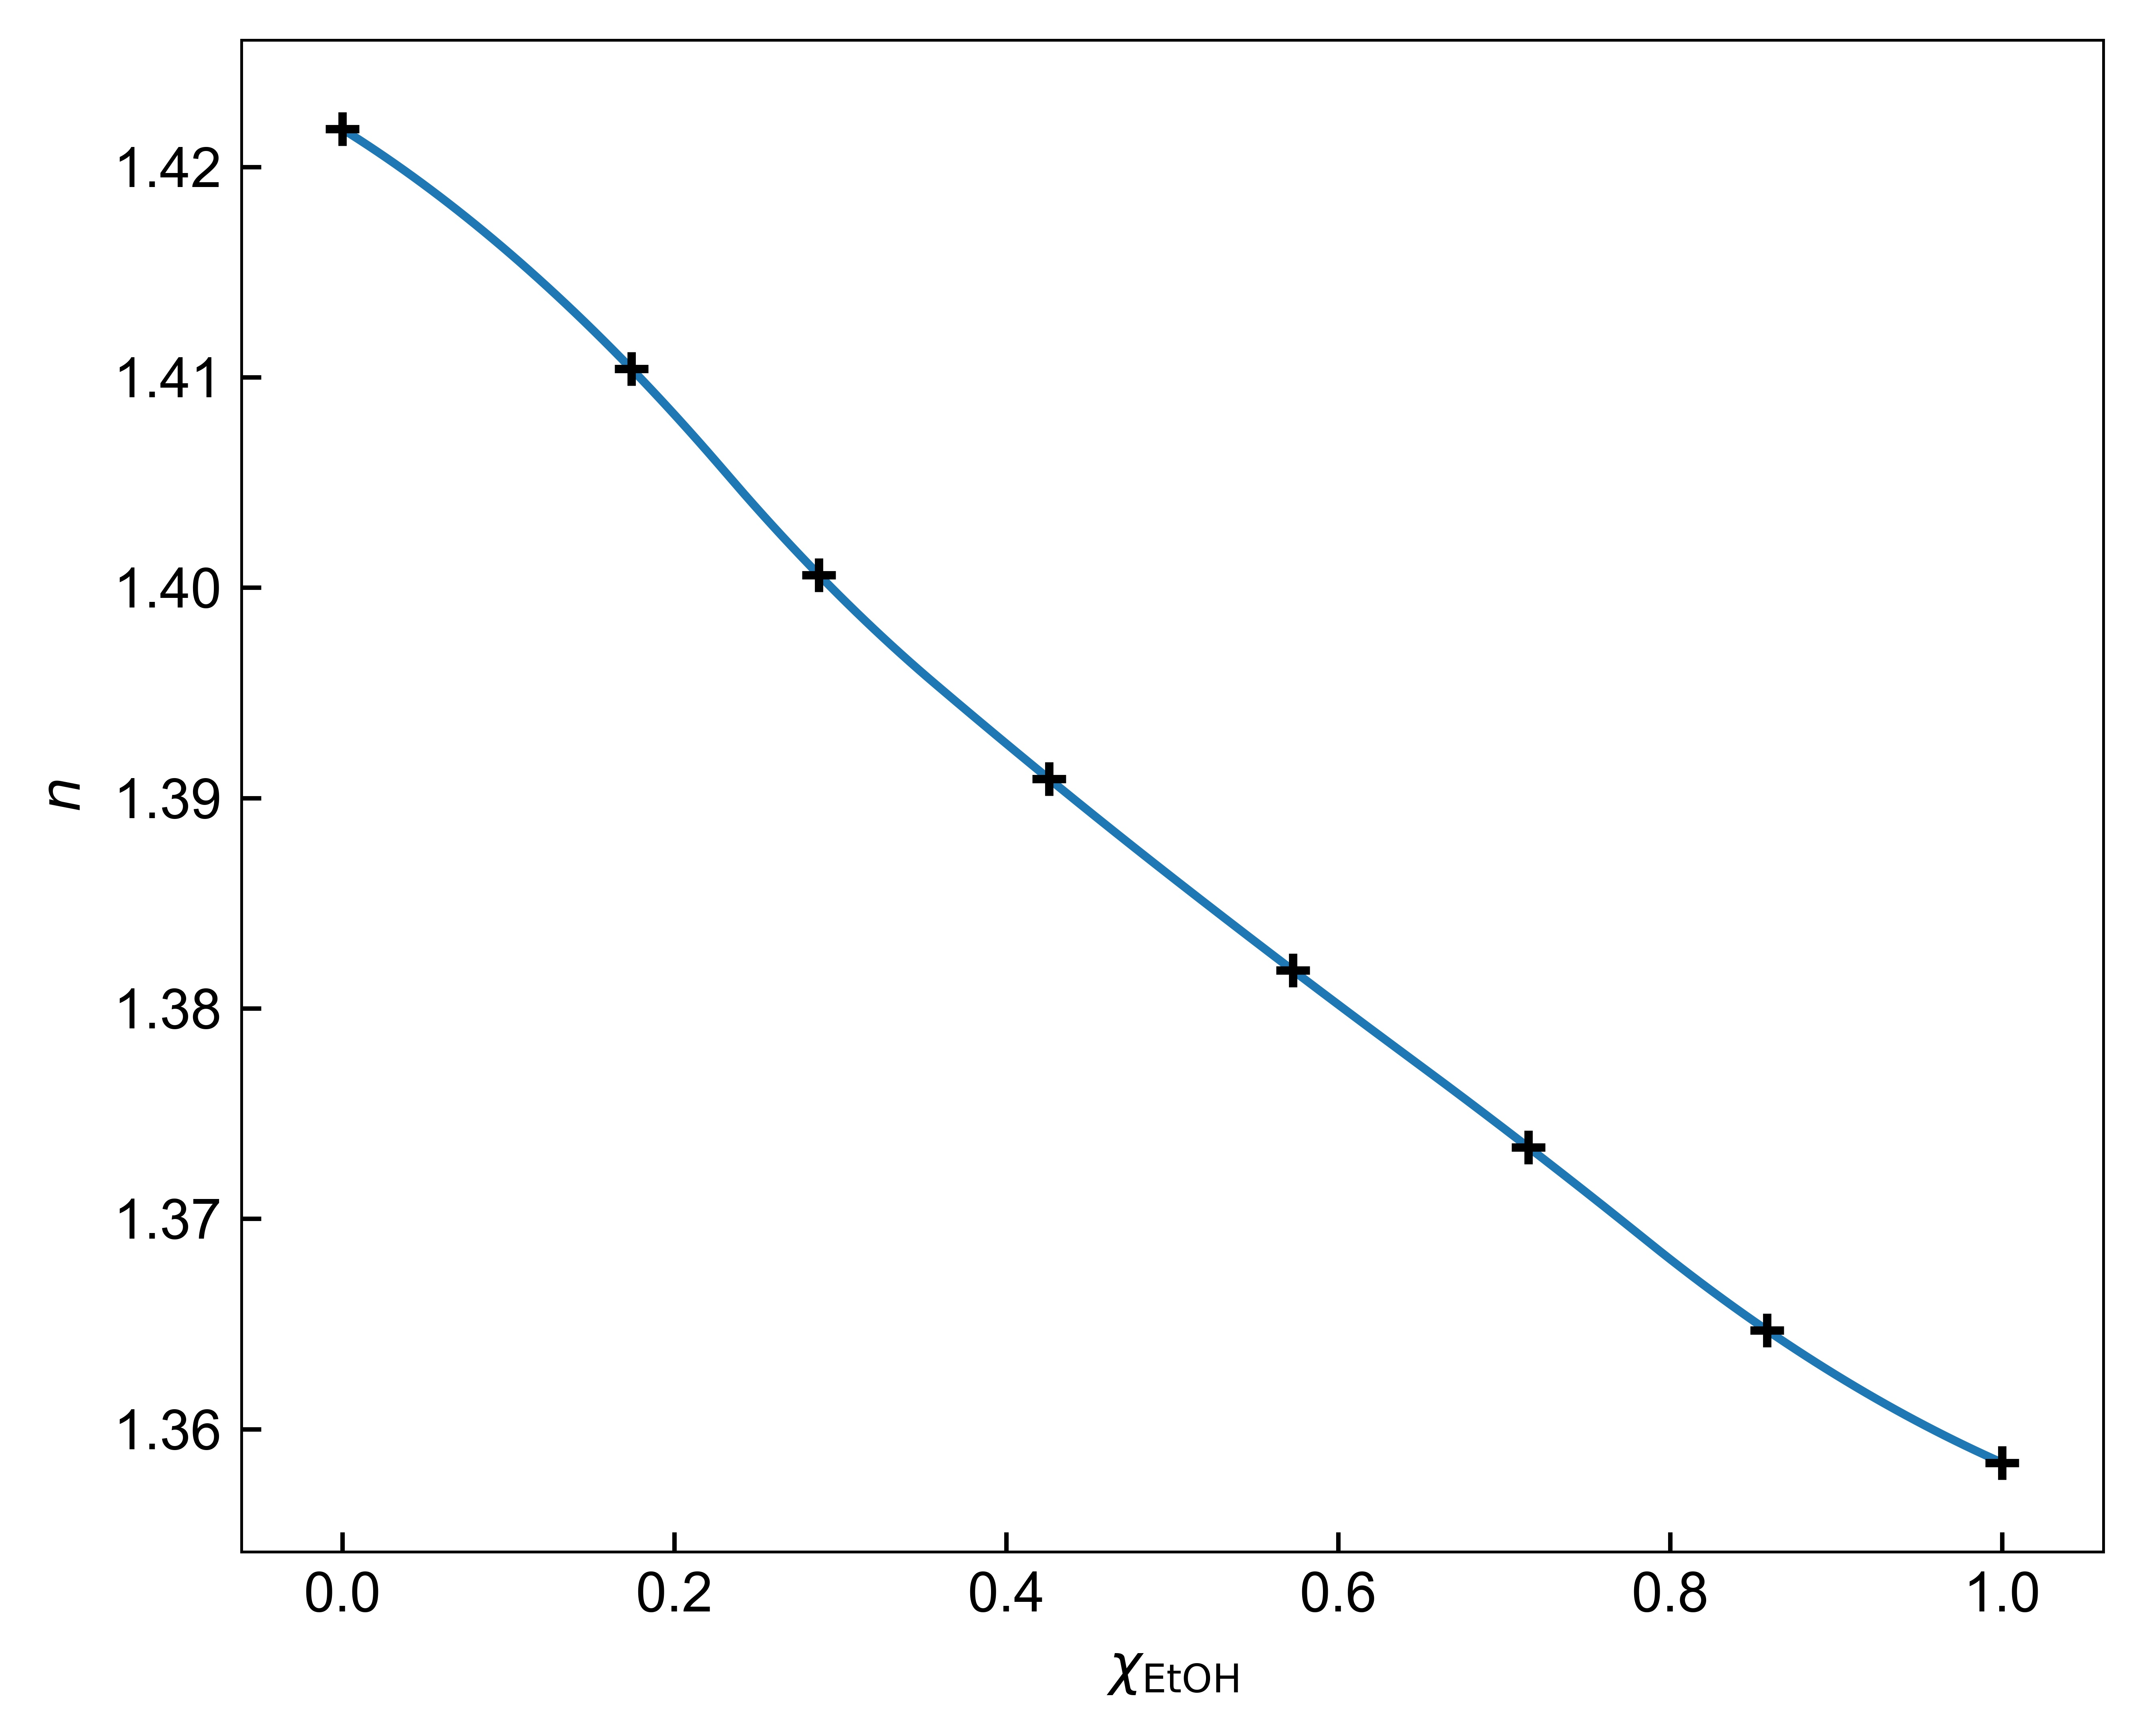
\includegraphics[width=0.55\textwidth]{1.jpg}
	\bicaption{乙醇-环己烷体系$n-\chi_{\ce{EtOH}}$标准工作曲线}{$n-\chi_{\ce{EtOH}}$ Standard working curve of ethanol-cyclohexane system}
\end{figure}
\par



 \subsection{数据处理结果与分析}
 \subsubsection{气液平衡时液相、气相组成计算}
根据\textbf{图1}二次函数插值得到的$n-\chi_{\ce{EtOH}}$标准工作曲线,将\textbf{表1}、\textbf{表2}中的液相折射率$n^{l}$、气相折射率$n^{g}$换算成对应的液相中乙醇质量分数$\chi^{l}_{\ce{EtOH}}$、气相中乙醇质量分数$\chi^{g}_{\ce{EtOH}}$,结果如\textbf{表4}所示。
\begin{table}[h]
	\centering
	\zihao{5}
	\bicaption{乙醇-环己烷体系气液平衡时液相、气相组成计算数据}{Calculation data of liquid and gas phase composition of EtOH-Cy at gas-liquid equilibrium}
	\begin{tabular}{cccccc}
		\toprule
		编号 & $t_{b}/{\rm ^{\circ}C}$ & $n^{l}$ & $n^{g}$ & $\chi^{l}_{\rm EtOH}$ & $\chi^{g}_{\ce{EtOH}}$ \\
		\midrule
	1 & 78.19 & 1.3584 & 1.3582 & 1.00 & 1.00 \\
	2 & 75.30 & 1.3601 & 1.3746 & 0.96 & 0.69 \\
	3 & 73.35 & 1.3632 & 1.3850 & 0.89 & 0.52 \\
	4 & 70.45 & 1.3668 & 1.3915 & 0.82 & 0.42 \\
	5 & 67.92 & 1.3732 & 1.3950 & 0.72 & 0.36 \\
	6 & 66.43 & 1.3773 & 1.3964 & 0.65 & 0.34 \\
	7 & 65.72 & 1.3836 & 1.3977 & 0.54 & 0.33 \\
		\midrule
	1 & 80.30 & 1.4218 & 1.4216 & 0.00 & 0.00 \\
	2 & 78.29 & 1.4206 & 1.4024 & 0.02 & 0.27 \\
	3 & 74.16 & 1.4201 & 1.4007 & 0.03 & 0.29 \\
	4 & 68.21 & 1.4185 & 1.3999 & 0.06 & 0.30 \\
	5 & 66.68 & 1.4168 & 1.3995 & 0.08 & 0.30 \\
	6 & 65.22 & 1.4106 & 1.3990 & 0.17 & 0.31 \\
	7 & 64.89 & 1.3996 & 1.3986 & 0.30 & 0.31 \\
	8 & 65.06 & 1.3927 & 1.3984 & 0.40 & 0.32 \\	
		\bottomrule
	\end{tabular}
\end{table}
\par

\subsubsection{乙醇-环己烷体系沸点-气、液成分图}
近似认为实验过程中大气压恒为$p=101.97\ \ {\rm kPa}$,溶液沸点在恒定压强下测得。根据\textbf{表4}数据,以气相、液相中乙醇质量分数$\chi_{\ce{EtOH}}$为横坐标,平衡沸点$t_{b}$为纵坐标,绘制乙醇-环己烷体系的沸点-成分图,如\textbf{图2}所示。
\begin{figure}[h]
	\centering
	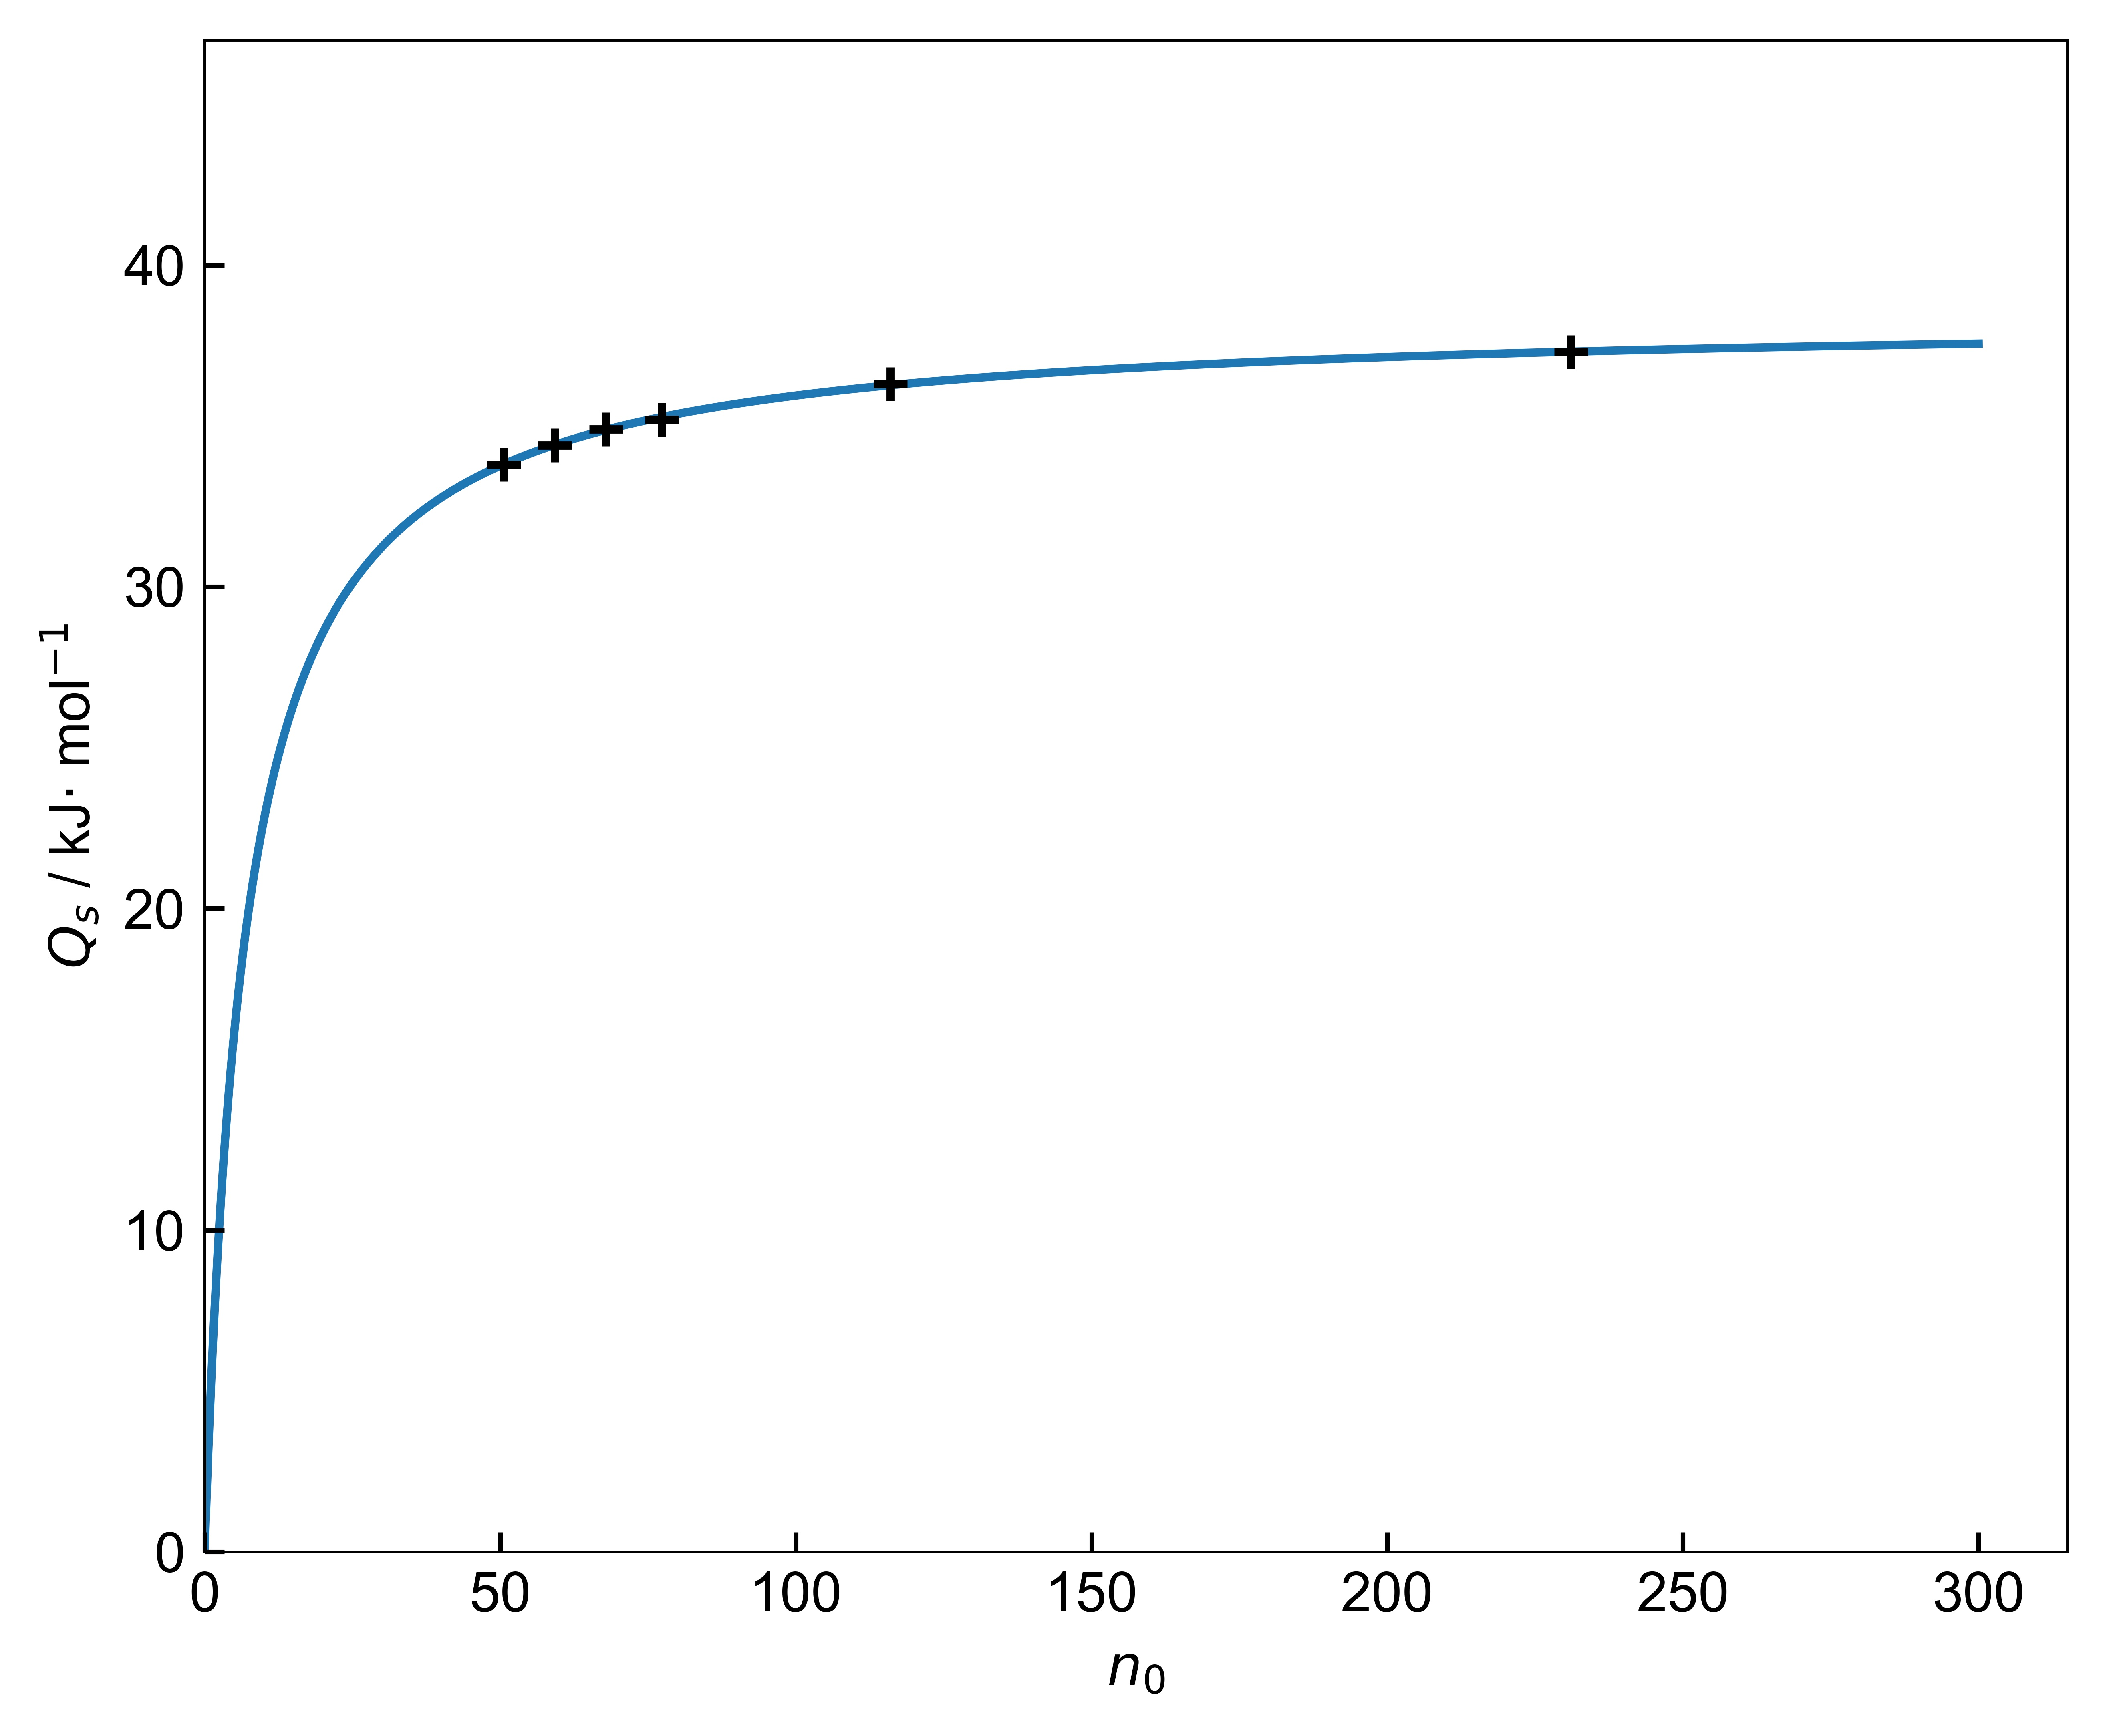
\includegraphics[width=0.55\textwidth]{2.jpg}
	\bicaption{乙醇-环己烷体系沸点-气、液成分图}{Boiling point-gas and liquid phase composition diagram of ethanol-cyclohexane system}
\end{figure}
\par
根据\textbf{图2},读出乙醇-环己烷体系的恒沸点为$t_{b}=64.97\ \ {\rm ^{\circ}C}$,组成为$\chi_{\ce{EtOH}}=0.31$。查阅\textit{CRC Handbook of Chemistry and Physics}\citealp{crc},知乙醇-环己烷体系在近常压$p_{0}=102.26\ \ {\rm kPa}$下的恒沸点为$T_{b}=337.95\ \ {\rm K}$即$t_{b}=64.80\ \ {\rm ^{\circ}C}$,组成为$\chi_{\ce{EtOH}}=0.4540$。实验测得乙醇-环己烷体系的恒沸点与文献参考值接近,但测得恒沸混合物组成严重偏离文献参考值,$\chi_{\ce{EtOH}}$显著小于文献给出的$\chi_{\ce{EtOH}}=0.4540$。

\vbox{}
 	 \section{讨论与结论}
		\subsection{实验讨论}
 			\subsubsection{标准工作曲线的绘制:拟合与插值的优劣}
 			在实验过程中,需要根据乙醇-环己烷体系的$n-\chi_{\ce{EtOH}}$工作曲线,由折射率$n$读出液相、气相组成。因此,$n-\chi_{\ce{EtOH}}$曲线绘制的准确性对实验误差有着相当程度的影响。下面对标准工作曲线的绘制进行简要讨论。\par 
 			在3.1.3中,使用二次函数插值作出乙醇-环己烷体系的$n-\chi_{\ce{EtOH}}$工作曲线。但根据\textbf{图1}可以看出,按此方法作出的标准工作曲线由于在不同区间上具有不同的表达式,因此在不同区间上具有不同的凹凸性和形状;并且实验中每个$\chi_{\ce{EtOH}}$下仅配制一次标准溶液样品、测定一次样品折射率,不可避免地存在一定程度误差,而通过插值作出的标准工作曲线需要过每一个数据点,误差较大的数据点对该点附近曲线会造成很大影响,使得作出的$n-\chi_{\ce{EtOH}}$曲线在一定范围内相当程度地偏离真实值。\par 
 			查阅相关文献\citealp{wenxian1},知乙醇-环己烷体系的$n-\chi_{\ce{EtOH}}$工作曲线可以很好地用二次函数进行拟合。依此方法作出乙醇-环己烷体系的$n-\chi_{\ce{EtOH}}$标准工作曲线,如\textbf{图3}所示。
 		\begin{figure}[h]
 			\centering
 			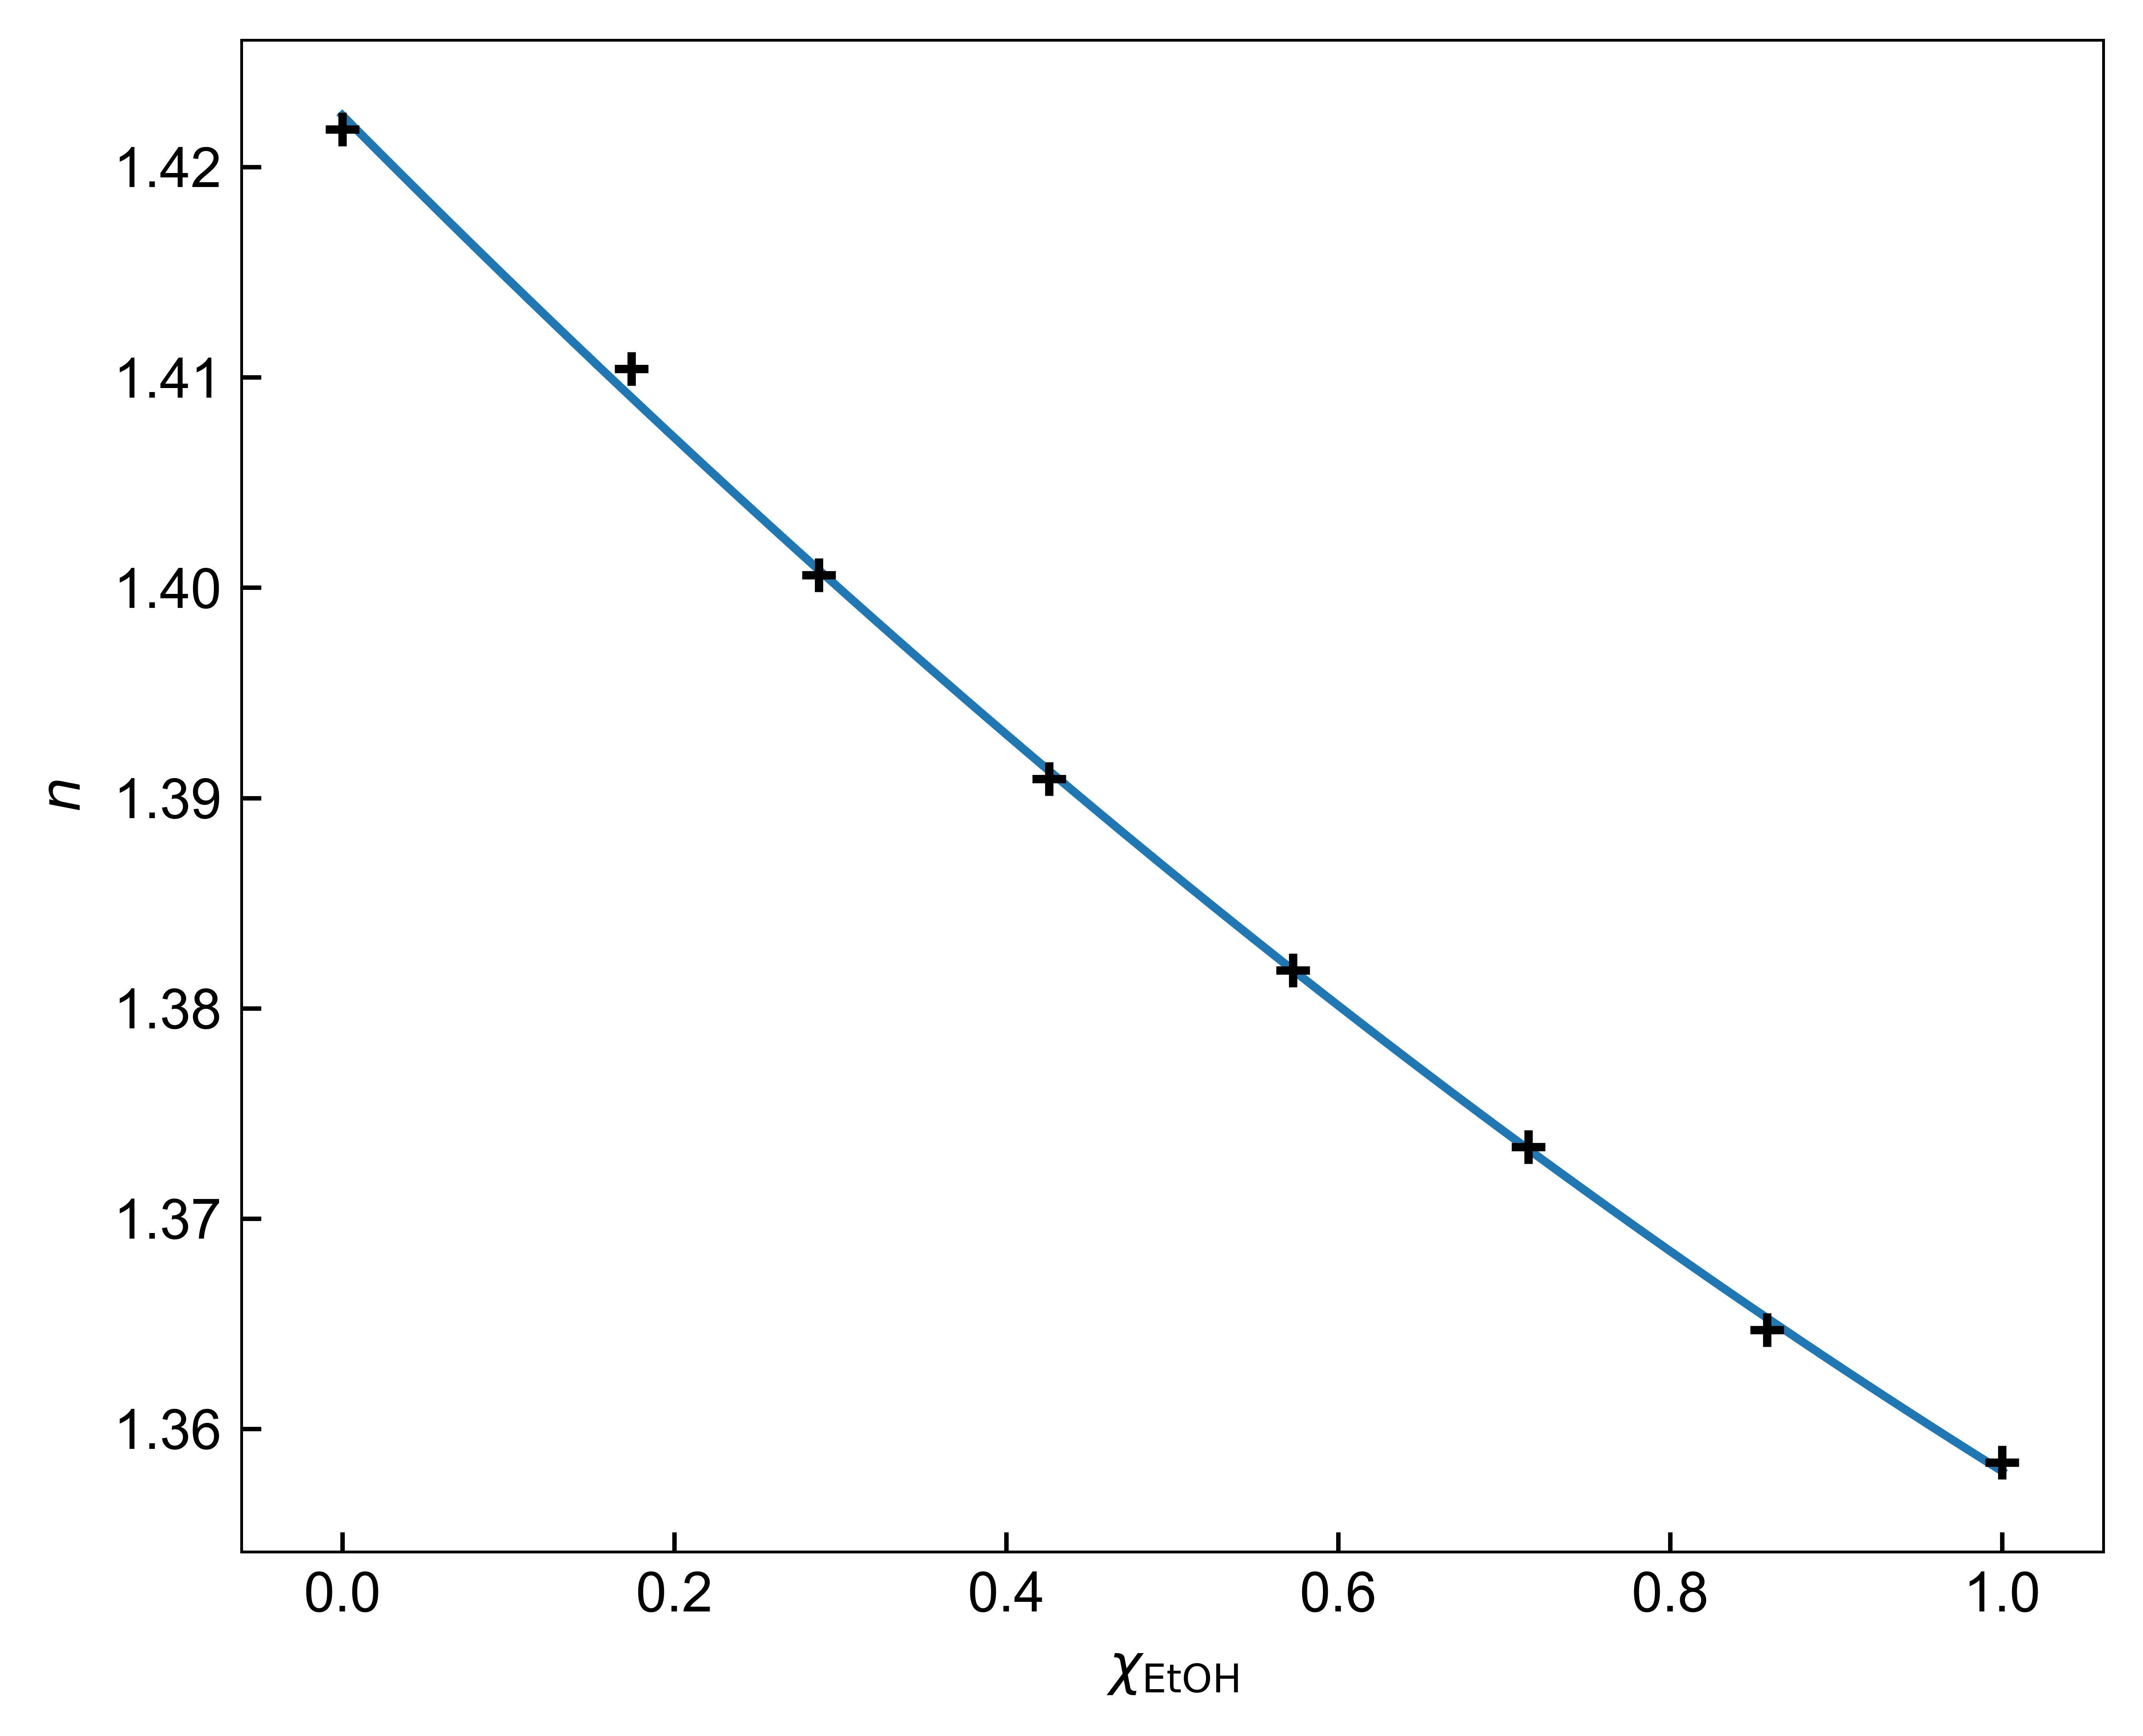
\includegraphics[width=0.6\textwidth]{3.jpg}
 			\bicaption{乙醇-环己烷体系$n-\chi_{\ce{EtOH}}$标准工作曲线(二次函数拟合)}{$n-\chi_{\ce{EtOH}}$ Standard working curve of ethanol-cyclohexane system (quadratic function fitting)}
 		\end{figure}
 		\par
 		拟合曲线的方程为
 		$$
 		n=(0.015\pm 0.002)\chi^{2}_{\ce{EtOH}}-(0.080\pm 0.003)\chi_{\ce{EtOH}}+(1.4224\pm 0.0007),\  \ R^{2}=0.99914
 		$$
 		根据\textbf{图3}可以看出,二次函数拟合得到$n-\chi_{\ce{EtOH}}$工作曲线收到了很好的效果,各个数据点基本落在拟合曲线上。可以判断,在本次实验中,使用曲线拟合相比使用插值法受到单个数据点误差的干扰更小,因此能够更有效地减小误差、作出更准确的$n-\chi_{\ce{EtOH}}$标准工作曲线。
 	\par 
 	\subsubsection{$n-\chi_{\ce{EtOH}}$非线性的原因分析}
		$n-\chi_{\ce{EtOH}}$标准工作曲线不具有线性的形式,下面结合理论推导作一简要分析。\par 查阅文献可知\citealp{wenxian2},在一定温度下,物质的折射率$n$与摩尔浓度$c$呈线性关系,即
		$$
		n=kc+A
		$$
		其中,理论上$A=1$,$k$为与入射光波长$\lambda$及物质本身性质有关的常数。假设实验中实际的乙醇-环己烷体系仅由乙醇、环己烷两相组成,记乙醇、环己烷摩尔质量之比
		$$
		\xi=\frac{M_{\rm EtOH}}{M_{\rm Cy}}=0.5474
		$$
		则理论上的折射率
		$$
		n=k_{1}\frac{\chi_{\ce{EtOH}}}{\chi_{\ce{EtOH}}+\xi (1-\chi_{\ce{EtOH}})}+k_{2}\frac{\xi (1-\chi_{\ce{EtOH}})}{\chi_{\ce{EtOH}}+\xi (1-\chi_{\ce{EtOH}})}+c
		$$ 		
		根据以上表达式的形式,使用python SciPy optimize进行拟合,作出乙醇-环己烷体系的$n-\chi_{\ce{EtOH}}$标准工作曲线,如\textbf{图4}所示。
		\begin{figure}[h]
			\centering
			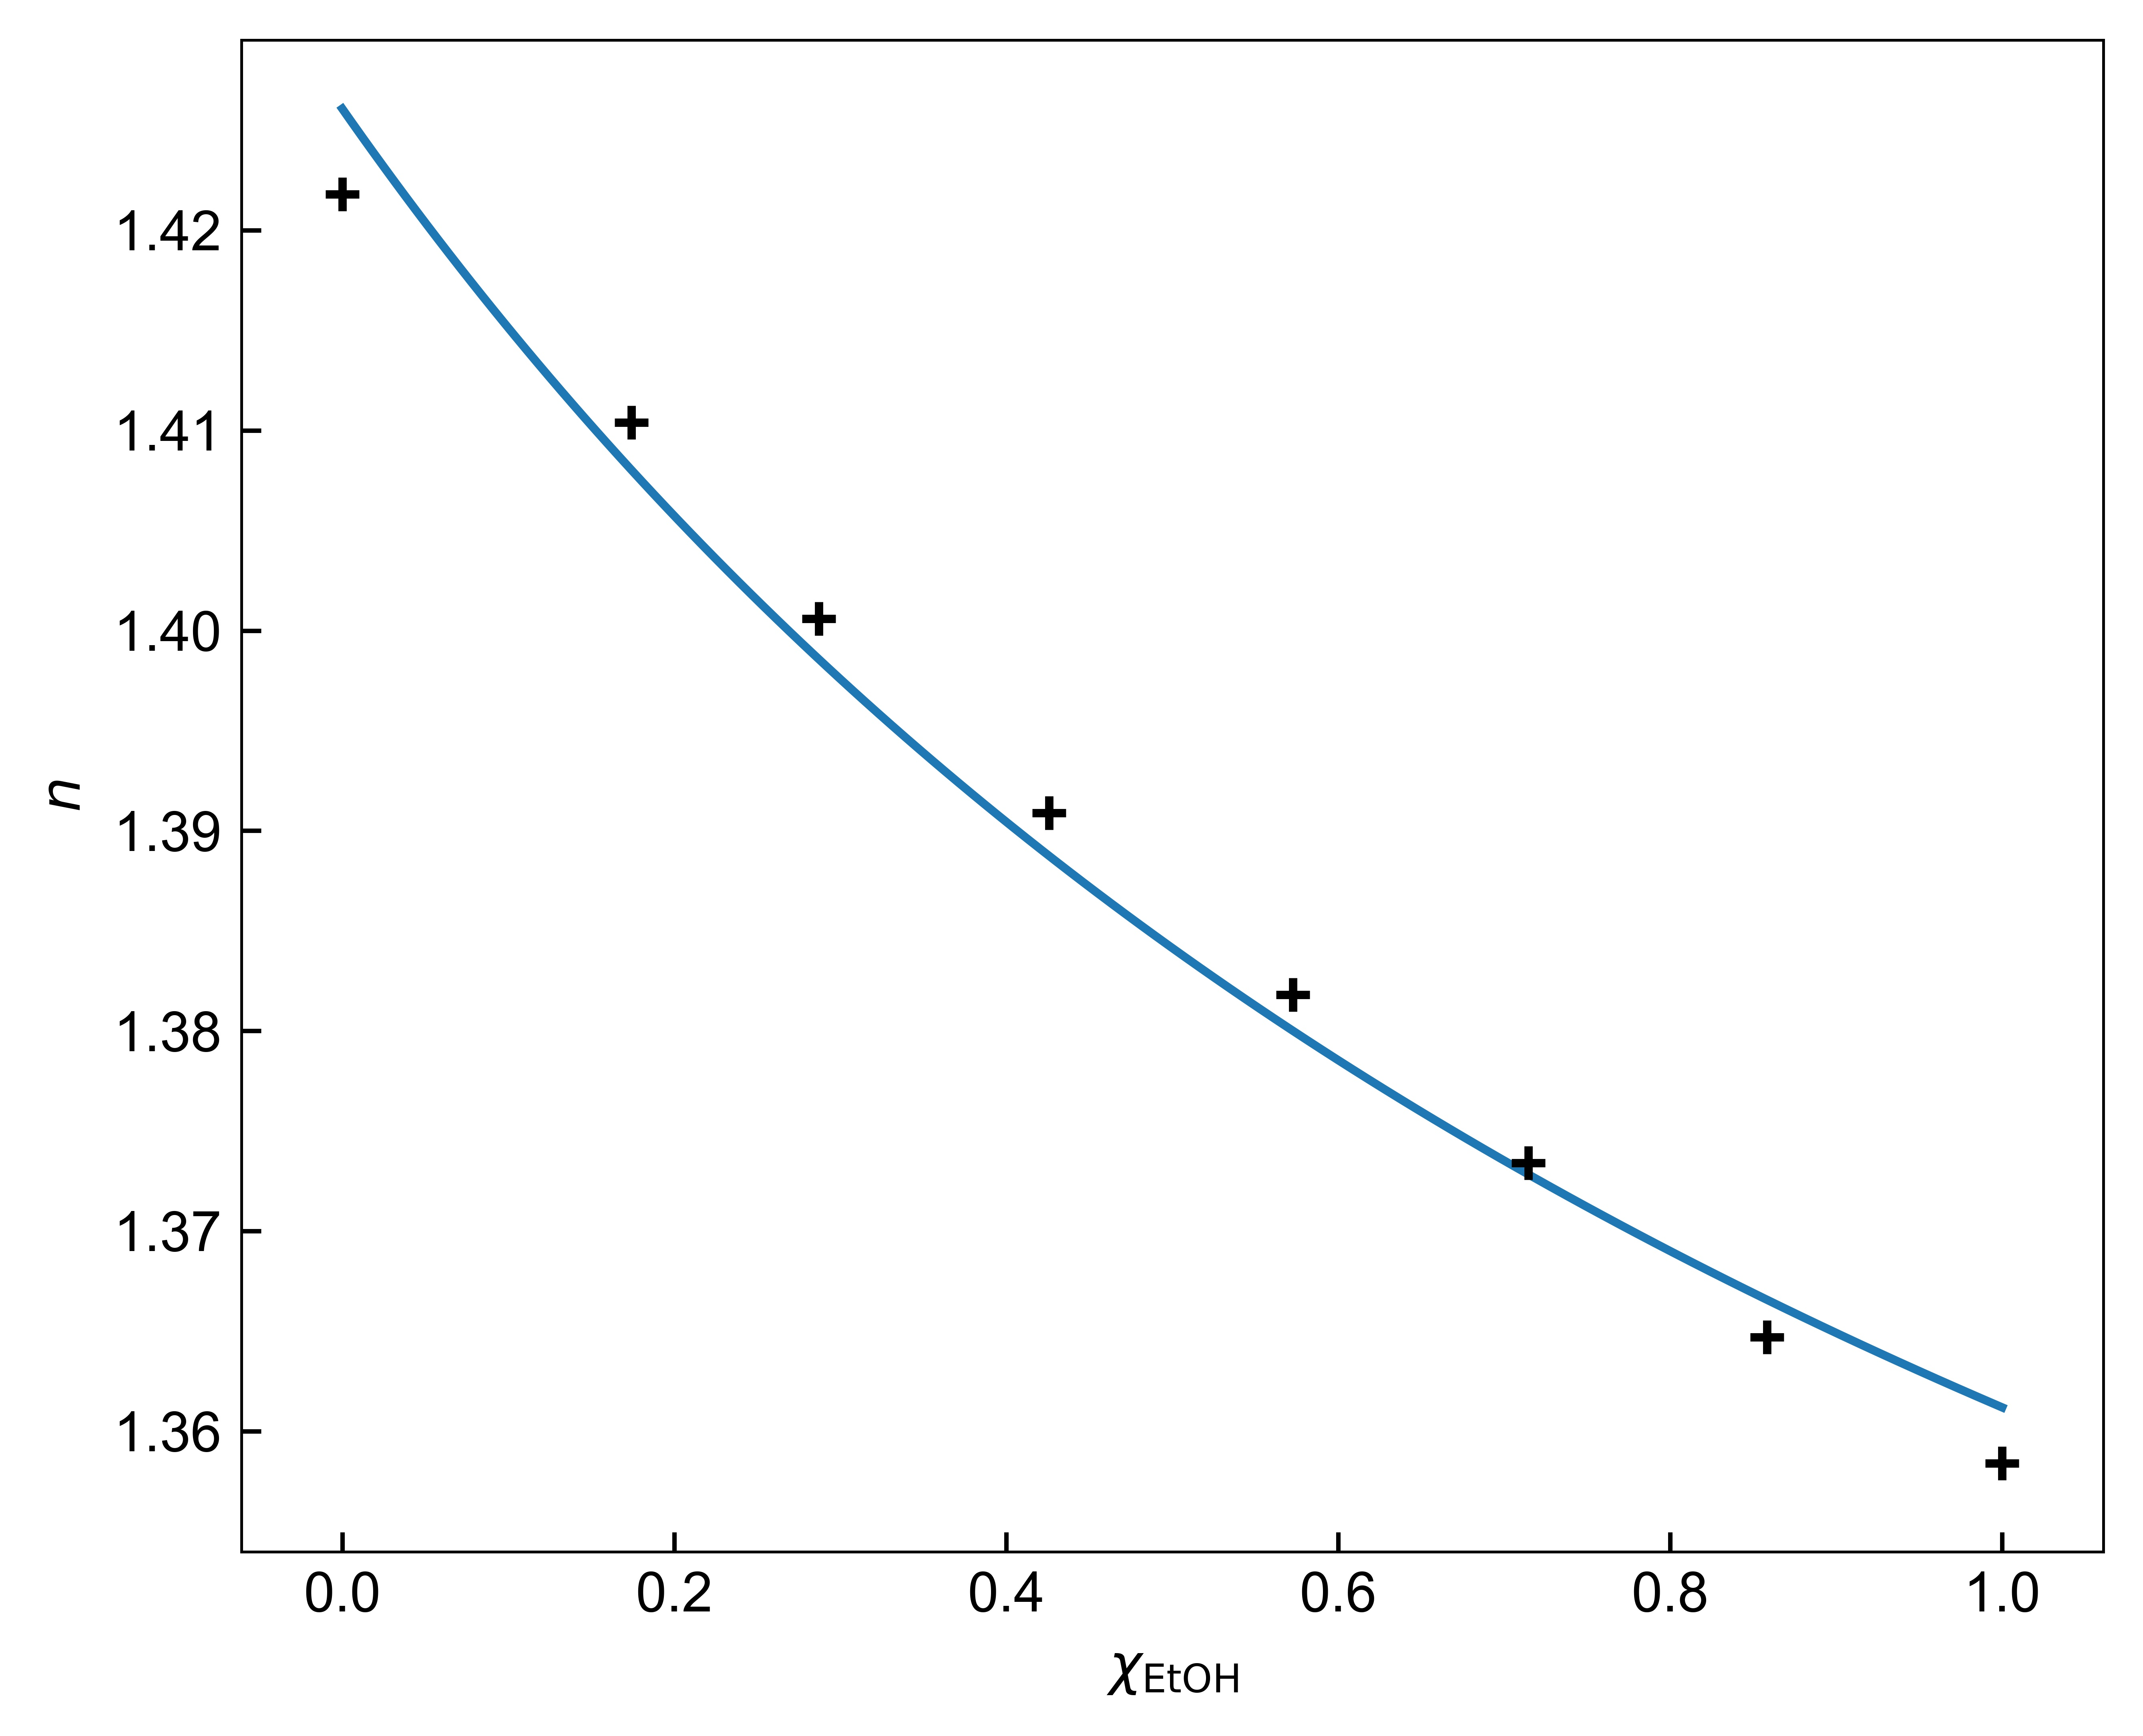
\includegraphics[width=0.6\textwidth]{4.jpg}
			\bicaption{乙醇-环己烷体系$n-\chi_{\ce{EtOH}}$标准工作曲线(理论公式拟合)}{$n-\chi_{\ce{EtOH}}$ Standard working curve of ethanol-cyclohexane system (theoretical formula fitting)}
		\end{figure}
		\par
		可见理论公式较好地与实验相符合,但仍有一定的差异。经分析,该差异可能是由于实验所用的乙醇中混有少量的水,从而对乙醇-环己烷体系实际的$n-\chi_{\ce{EtOH}}$工作曲线造成了影响。
 			\subsubsection{实验改进}
 			实际实验中,由于加热用的电阻丝位于蒸馏烧瓶底部,且整个系统保温较差,蒸馏烧瓶内存在自下而上的温度梯度,靠近电阻丝的部分温度较高,而远离电阻丝的冷凝管处温度显著较低,且冷凝管内也存在自下而上的温度梯度,产生了显著的分馏现象,从而使得所测得的液相组分并非测量温度下的实际组分,造成了一定的实验误差,可能因此导致了恒沸混合物$\chi_{\ce{EtOH}}$与文献参考值的严重偏离。\par 
 			相应的改进:装置加装恒温水浴保温装置,消除蒸馏烧瓶及冷凝管内的温度梯度。
 		



 	 \subsection{实验结论}
 	 本实验采用回流冷凝法测定了不同浓度乙醇-环己烷体系的沸点和气相、液相折射率,作出$n-\chi_{\ce{EtOH}}$工作曲线,计算了各平衡沸点下的两相组成,绘制了乙醇-环己烷体系沸点-成分图,确定了恒沸点$t_{b}=64.97\ \ {\rm ^{\circ}C}$,组成为$\chi_{\ce{EtOH}}=0.31$。\par 
 	 讨论了插值和拟合作出标准工作曲线的区别、标准工作曲线非直线的原因,利用二次函数重新拟合得到$n-\chi_{\ce{EtOH}}$标准工作曲线,并讨论了实验测得恒沸混合物$\chi_{\ce{EtOH}}$偏离文献参考值的原因,提出了一定的实验改进。



 

   

\vbox{}

\bibliographystyle{achemso}
\bibliography{b}



\end{document}